% Scale study: where the macro quantities of a citation graph stop fluctuating.
\documentclass[11pt]{article}
\usepackage[T1]{fontenc}
\usepackage{lmodern}
\usepackage{microtype}
\usepackage[margin=1in]{geometry}
\usepackage{amsmath,amssymb,amsthm,mathtools}
\usepackage{algorithm}
\usepackage{algpseudocode}
\usepackage{booktabs}
\usepackage{pgfplots}
\pgfplotsset{compat=1.17}
\usepackage[numbers,sort&compress]{natbib}
\usepackage[hidelinks]{hyperref}
\usepackage[capitalise,noabbrev]{cleveref}

\title{Where the Macro Quantities of a Growing Citation Graph Stop Fluctuating}
\author{Alberto Serrano-Calva}
\date{\today}

\begin{document}
\maketitle

\begin{abstract}
A macro description of an evolving graph is useful only when the quantities it uses stop fluctuating
under resampling, and theory names two thresholds: a time average needs a window of many relaxation
times $1/\gamma$, where $\gamma$ is the spectral gap of the normalized Laplacian, and the Laplacian's
eigenvalues concentrate once degrees exceed about $\log N$. We measure where these thresholds fall
on real data. The graph is the citation network of the OpenAlex concept Complex network, 47,546
works and 327,978 citations among them, grown by yearly date cuts to 33,342 nodes in its
largest component. At each cut we compute the smallest 20 eigenvalues, bootstrap $\gamma$ and the
first eigengaps by node subsampling and edge resampling, and split the time-oriented citation flow
into gradient, curl and harmonic energy with the same bootstrap. On the whole component the 95\%
interval of $\gamma$ is never within 10\% of its median at any scale up to 25,000 nodes, although
the mean degree is about $2\log N$ or more from the 2002 cut on: small groups joined to the rest by a single
citation set the gap, and the minimum degree is 1. On the 6-core and 10-core, whose minimum degrees
are 6 and 10, the interval of $\gamma$ under edge resampling is within 10\% from about 1,000 and
2,000 nodes (replicate size), where the minimum degree is 0.9 to 1.3 times $\log N$. The relaxation time $1/\gamma$ (continuous time) of the
whole component is 90 to 220, and a 10\% average needs $T_c = 17{,}000$ to $44{,}000$ in continuous time, or $T = 35{,}000$ to $87{,}000$ lazy steps at laziness $1/2$,
1.3 to 11 times $N$; for the cores $1/\gamma$ is 3 to 10 and $T$ about 1,300 to 4,000 lazy steps. The Hodge energies settle at 0.80 to
0.83 gradient, 0.15 to 0.18 curl and under 0.03 harmonic, and their widths fall under 10\% one to
two decades of $N$ below the scale for $\gamma$. A synthetic graph of 38 nodes and 20 edges in one generation is a forest
of 18 components, whose spectral gap is zero and whose windows are infinite. The code is generic over
any temporal edge list and is tested on graphs with known spectra.
\end{abstract}

\section{Introduction}
A graph that grows by the addition of nodes and edges can be summarized by a few macro quantities:
its size, degrees, the low end of the spectrum of its normalized Laplacian, and the split of an edge
flow into gradient, curl and harmonic parts. A macro model that uses these quantities is trustworthy
only if they do not move when the graph is perturbed in ways that leave its character unchanged, and
only if they are measured over a long enough window. Theory gives two statements about when that
holds. First, a time average of a macro observable along a random walk on the graph has a variance
governed by the relaxation time $1/\gamma$, so the window must be many relaxation times. Second, a
$k$-mode macro model is valid only after a time set by the gap between the $k$th and $(k{+}1)$th
eigenvalues. A third statement is a cited theorem: the eigenvalues of the normalized Laplacian of a
random graph concentrate around those of its expected counterpart once the degrees exceed about
$\log N$ \citep{oliveira2009,chungradcliffe2011}.

These statements have constants and conditions that the theory does not fix for a real graph. This
article measures them on one real evolving graph and reports where the thresholds fall in practice.
The contributions are:
\begin{itemize}
  \item a generic, tested procedure that takes any temporal edge list, grows the graph by date cuts,
  and reports size, degrees, the smallest 20 normalized-Laplacian eigenvalues, the spectral gap, the
  eigengaps, bootstrap interval widths, relaxation times, required windows and the Hodge split of
  an oriented flow;
  \item measurements on the citation network of one OpenAlex field up to 33,342 nodes, including the
  curve of interval width against scale, not only the crossing of a threshold;
  \item the observation that the degree condition of the theorem is a condition on the minimum
  degree, and that on the whole citation graph, where it is 1, no tested scale suffices, while on the
  cores, where it is of order $\log N$, the scale is about 1,000 to 2,000 nodes;
  \item the contrast with a graph of the size and shape of a small personal corpus, which lies
  below every threshold.
\end{itemize}

\section{Background and related work}
\paragraph{Data.} OpenAlex is an open index of scholarly works, authors, venues, institutions and
concepts released under CC0 \citep{priem2022openalex}. A work record carries its publication date
and the list of works it references, which is what a temporal citation graph needs.

\paragraph{Spectral graph theory.} For a graph with adjacency matrix $A$ and degree matrix $D$ the
normalized Laplacian is $\mathcal L = I - D^{-1/2} A D^{-1/2}$, with eigenvalues
$0 = \lambda_1 \le \lambda_2 \le \dots \le 2$ \citep{chung1997}. The spectral gap is
$\gamma = \lambda_2$. The simple random walk $P = D^{-1}A$ has eigenvalues $1 - \lambda_i$, so
$\gamma$ is its spectral gap. In continuous time the walk's relaxation time is $1/\gamma$; in discrete
steps it is set by the absolute spectral gap, which the lazy walk of \cref{sec:window} makes
$\varepsilon\gamma$ \citep{levin2017}. The
Cheeger inequality bounds $\gamma$ by the conductance of the best cut, so a set of nodes joined to
the rest by few edges forces $\gamma$ to be small \citep{chung1997}.

\paragraph{Concentration.} For random graphs with independent edges, the normalized Laplacian
concentrates around its expectation in operator norm when the minimum expected degree exceeds a
constant multiple of $\log N$ \citep{oliveira2009,chungradcliffe2011}. Both results assume a
random model. We use the degree condition only as a reference point: the question is where a real
graph, which is not a sample of such a model, behaves as the condition predicts.

\paragraph{Hodge decomposition of flows.} A flow on the edges of a graph, together with its
triangles (the clique complex), decomposes orthogonally into a gradient part, a curl part and a
harmonic part \citep{lim2020,jiang2011}. The gradient part is the projection onto flows of the form
$s_j - s_i$ for a node potential $s$; the curl part is the projection onto the image of the
transpose of the edge-to-triangle boundary operator; the harmonic part is the remainder. For a
citation flow the gradient energy measures how far citations follow a ranking of the works, and
the curl and harmonic energies measure inconsistency with any ranking.

\paragraph{Citation network growth.} The early model of the growth of a network of papers by
\citet{price1965} has new papers cite old ones with probability that increases with their existing
citations. We use no growth model; we use only the fact that citations point from newer to older
works.

\paragraph{Resampling.} The bootstrap of \citet{efron1979} estimates the spread of a statistic by
recomputing it on resampled data. Here the resampled objects are graphs, resampled by nodes and by
edges, and the statistic is a spectral quantity.

\section{Data and method}
\subsection{The field}
The graph is the concept Complex network of OpenAlex (identifier C34947359; OpenAlex reported about
47,700 works for it on 2026-11-07). The field was chosen because it is coherent, begins in 1998,
and is small enough to fetch in minutes while reaching more than $3\times 10^4$ connected nodes.
Nodes are works with a publication date. An edge $u \to v$ means that $u$ cites $v$, kept only when
both works are in the field; its time is the publication date of $u$. The stored graph has 47,546
works and 327,978 such citations. Raw pages (293 files of up to 200 works, 31 MB compressed) and
derived files total 41 MB, kept outside the repository.

The fetch used the \texttt{/works} endpoint with \texttt{select} limited to the identifier, the
publication date, the referenced works and the concepts. Cursor paging past the first page requires
an API key, which this study did not obtain, so the field was cut into date ranges of at most
9,000 works (a range is halved until it fits under the limit of basic paging) and each range was
read with page numbers. Requests were sequential with a 0.5 second pause and a User-Agent naming the
project; errors were retried with exponential backoff and a rerun skips pages already stored.

\subsection{Growth by cuts}
\Cref{alg:cuts} grows the graph. For each cut time $t$ the graph is the set of edges dated at or
before $t$, symmetrized, without loops or duplicate edges, restricted to its largest connected
component. Cuts are at 31 December from 1995 to 2024 and at 2025-12-31 and 2026-11-07.

\begin{algorithm}
\caption{Growth by cuts and measurement.}\label{alg:cuts}
\begin{algorithmic}[1]
\Require temporal edges $(u,v,t)$ sorted by $t$; cut times $T$; core orders $K$
\For{each cut $t \in T$}
  \State $E_t \gets$ edges with time $\le t$; $G_t \gets$ largest component of symmetrize$(E_t)$
  \State record $N$, mean degree $\bar d$, minimum degree $d_{\min}$ and $\bar d/\ln N$ of $G_t$
  \State $\lambda_1,\dots,\lambda_{20} \gets$ smallest eigenvalues of $\mathcal L(G_t)$; $\gamma \gets \lambda_2$
  \State record $1/\gamma$, $T_c = 2/(\gamma\delta^2)$ and $T = T_c/\varepsilon$ with laziness $\varepsilon = 1/2$
  \State Hodge split of the flow of $G_t$ (gradient, curl, harmonic fractions)
  \State bootstrap $G_t$ (\Cref{alg:boot}); for each $k \in K$ repeat on the $k$-core of $G_t$
\EndFor
\end{algorithmic}
\end{algorithm}

\subsection{Spectrum}
Up to 500 nodes the eigenvalues come from a dense symmetric solver. Above that they come from
\texttt{scipy.sparse.linalg.eigsh} in shift-invert mode with shift $\sigma = -0.01$, \texttt{which=LM},
tolerance $10^{-8}$, and a sparse LU factorization of $\mathcal L + 0.01 I$ under a minimum-degree
ordering supplied as the inverse operator \citep{lehoucq1998}. The ordering matters: the default
ordering took 162 seconds at 21,681 nodes and the minimum-degree ordering about 10 seconds. The
eigengaps are $\lambda_{k+1} - \lambda_k$, so the first equals $\gamma$.

\subsection{Bootstrap}
\Cref{alg:boot} resamples a component by nodes or by edges. A node sample of fraction $p$ keeps the
subgraph induced by $\lceil pN \rceil$ uniformly chosen nodes. An edge sample draws $m$ edges with
replacement from the $m$ edges, which keeps about 63\% of the distinct edges. Each replicate is
reduced to its largest component and, for the core analysis, to the largest component of its
$k$-core. The relative width of the 95\% interval of a statistic is
$(q_{97.5} - q_{2.5}) / |q_{50}|$ over the replicates. The scale of a row is the mean $N$ of its
replicates. We use 20 replicates for the spectral statistics and 6 for the Hodge fractions. The
crossing scale $N^{*}$ is the smallest scale from which the width is at most 10\% at every larger
scale measured. Whole-component bootstraps were run up to 25,000 nodes and core bootstraps up to
15,000.

\begin{algorithm}
\caption{Bootstrap of a component.}\label{alg:boot}
\begin{algorithmic}[1]
\Require component $G$, scheme (node fraction $p$, or edge), core order $k$, replicates $B$
\For{$b = 1,\dots,B$}
  \If{scheme is node}
    \State $H \gets$ largest component of $G[S]$, $S$ a uniform sample of $\lceil pN\rceil$ nodes
  \Else
    \State $H \gets$ largest component of the graph on $m$ edges drawn with replacement from $E(G)$
  \EndIf
  \If{$k > 1$} \State $H \gets$ largest component of the $k$-core of $H$ \EndIf
  \State compute $N_b$, $\gamma_b$ and the eigengaps of $H$
\EndFor
\State \Return for each statistic, $(q_{97.5}-q_{2.5})/|q_{50}|$ over $b$, and the mean of $N_b$
\end{algorithmic}
\end{algorithm}

\subsection{Relaxation and window}\label{sec:window}
SCL-1 of the companion article on scale and attribution is proved for the lazy walk
$x \mapsto (1 - \varepsilon L)x$ of the combinatorial Laplacian $L = D - A$, with laziness $\varepsilon$
and $\varepsilon\lambda_{\max} \le 1$. Its argument uses only that the operator is symmetric with
spectrum in $[0, 1/\varepsilon]$ and that the field is orthogonal to the kernel, so it holds as stated
for $1 - \varepsilon\mathcal L$ with $x \perp D^{1/2}\mathbf 1$; the machine-checked statement covers $L$
only. The lazy random walk $(1-\varepsilon)I + \varepsilon P = D^{-1/2}(I - \varepsilon\mathcal L)D^{1/2}$
has the same eigenvalues $1 - \varepsilon\lambda_i$ and is reversible for the degree-weighted
distribution $\pi$. The spectrum of $\mathcal L$ lies in $[0,2]$, so the largest admissible laziness
is $\varepsilon = 1/2$, which we use. The deterministic bound is that the energy of
the time average over $T$ steps of a mean-zero field $x$ is at most $\|x\|^2/(T\varepsilon\gamma)^2$. For an
observable read along the lazy random walk started from $\pi$, the sampled form, here the textbook
bound for a reversible chain \citep{levin2017} with $\sigma^2$ the variance under $\pi$, is
$\mathrm{Var} \le 2\sigma^2/(\varepsilon\gamma T)$ per lazy step, and
$\mathrm{Var} \le 2\sigma^2/(\gamma T_c)$ in continuous time $T_c = \varepsilon T$. A relative precision
$\delta$ of an observable of unit relative standard deviation therefore needs, in the two unit systems,
\[
T = \frac{2}{\varepsilon\gamma\delta^2}\ \text{lazy steps}, \qquad T_c = \varepsilon T = \frac{2}{\gamma\delta^2}.
\]
At $\varepsilon = 1/2$ and $\delta = 0.1$ these are $T = 400/\gamma$ and $T_c = 200/\gamma$. The relaxation time
is $1/\gamma$ in continuous time and $1/(\varepsilon\gamma) = 2/\gamma$ in lazy steps. We report both;
$1/\gamma$ and $T_c$ are continuous time, $1/(\varepsilon\gamma)$ and $T$ lazy steps.

\subsection{Hodge split}
The flow on a canonical edge $\{i<j\}$ is $+1$ if $i$ cites $j$, $-1$ if $j$ cites $i$, and $0$ for a
mutual pair. The clique complex has all triangles of the symmetrized component. The gradient and
curl projections are computed by LSMR (tolerance $10^{-8}$) and the harmonic energy is the
remainder. Energies are reported as fractions of the squared norm of the flow.

\section{Results}
\subsection{The graph as it grows}
\Cref{tab:cuts} lists selected cuts. The component grows from 43 nodes (2000) to 33,342 (2026); the mean
degree is 18 to 21 from 2007 on, so $\bar d/\ln N$ falls from 2.3 to 1.9. The minimum degree is 1 at
every cut: a citation graph built from truncated reference lists has works with one in-field
reference or one in-field citation. The volume of the last two years (3,795 works dated 2025 and
7,575 dated 2026, against 1,205 in 2024) is an indexing effect, and cuts after 2024 are shown for
completeness only.

\begin{table}[t]
\centering
\caption{Selected cuts of the largest component. $\gamma$ is $\lambda_2$ of the normalized
Laplacian. $1/\gamma$ and $T_c = 200/\gamma$ are in continuous time; $T = T_c/\varepsilon = 400/\gamma$ is in
lazy steps (SCL-1, $\varepsilon = 1/2$, precision $\delta = 10\%$).}\label{tab:cuts}
\begin{tabular}{lrrrrrrrr}
\toprule
cut & $N$ & $\bar d$ & $d_{\min}$ & $\bar d/\ln N$ & $\gamma$ & $1/\gamma$ & $T_c$ & $T$ \\
\midrule
2000-12-30 & 43 & 5.30 & 1 & 1.41 & 0.2827 & 3.5 & 707 & 1415 \\
2002-12-31 & 305 & 13.07 & 1 & 2.28 & 0.0521 & 19.2 & 3838 & 7677 \\
2004-12-30 & 917 & 15.40 & 1 & 2.26 & 0.0760 & 13.2 & 2632 & 5264 \\
2006-12-31 & 2076 & 17.19 & 1 & 2.25 & 0.1153 & 8.7 & 1734 & 3469 \\
2008-12-30 & 3878 & 18.62 & 1 & 2.25 & 0.1496 & 6.7 & 1337 & 2675 \\
2009-12-30 & 5066 & 18.59 & 1 & 2.18 & 0.0073 & 136.3 & 27252 & 54504 \\
2012-12-30 & 8995 & 18.59 & 1 & 2.04 & 0.0075 & 133.8 & 26764 & 53528 \\
2015-12-31 & 14152 & 19.10 & 1 & 2.00 & 0.0046 & 218.6 & 43722 & 87444 \\
2018-12-31 & 19487 & 19.97 & 1 & 2.02 & 0.0081 & 123.0 & 24593 & 49186 \\
2021-12-31 & 24926 & 20.39 & 1 & 2.01 & 0.0074 & 135.6 & 27111 & 54221 \\
2024-12-30 & 28773 & 20.59 & 1 & 2.01 & 0.0094 & 105.9 & 21174 & 42348 \\
2026-11-07 & 33342 & 19.65 & 1 & 1.89 & 0.0089 & 112.0 & 22395 & 44790 \\
\bottomrule
\end{tabular}
\end{table}

\subsection{The spectral gap of the whole component does not concentrate}
The gap is 0.28 at 43 nodes, falls to about 0.05 by 2002, rises to 0.150 at the 2008 cut and then
falls by a factor of 20 to 0.0073 at the 2009 cut, where it stays between 0.005 and 0.012 up to
2026 (\Cref{fig:gamma}). A sweep cut on the Fiedler vector at the 2009 cut finds a set of 42 nodes
with volume 121 joined to the rest by one edge (conductance 0.008); at the 2026 cut it finds a set
of 7 nodes joined by one edge. The gap is set by small groups hanging on a single citation, as the
Cheeger inequality predicts for such a cut.

The bootstrap widths reflect this. The 95\% interval of $\gamma$ is wider than the median at most scales:
the median width over replicates is 1.3 to 4.2 for node subsampling and 0.5 to 6.0 for edge resampling,
with no downward trend from 10 to 25,000 nodes. Neither the width of $\gamma$ nor the widths of the
first four eigengaps ever stay within 10\% at any larger scale. The mean degree is about $2\ln N$ or more at
every cut from 2002 to 2024 (1.9 at the last), so the mean degree does not decide the matter; the minimum degree is 1, which is 0.1 to 0.3 of
$\ln N$.

\begin{figure}[t]
\centering
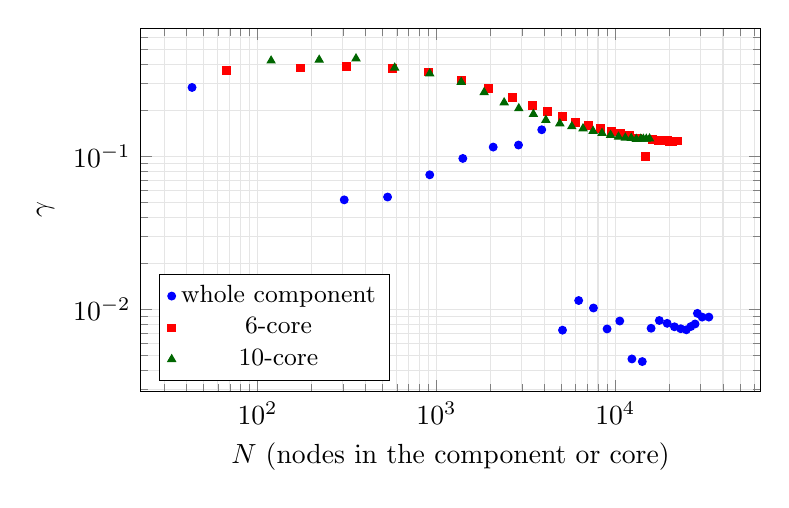
\begin{tikzpicture}
\begin{axis}[width=0.78\textwidth,height=6.2cm,xmode=log,ymode=log,xlabel={$N$ (nodes in the component or core)},
ylabel={$\gamma$},legend pos=south west,legend style={font=\small},grid=both,grid style={gray!20}]
\addplot[only marks,mark=*,mark size=1.4pt,blue] coordinates {(43,0.2827) (161,0.01525) (305,0.05211) (533,0.05438) (917,0.07598) (1404,0.09719) (2076,0.1153) (2876,0.1189) (3878,0.1496) (5066,0.007339) (6239,0.01146) (7549,0.01024) (8995,0.007473) (1.059e+04,0.00842) (1.238e+04,0.004758) (1.415e+04,0.004574) (1.585e+04,0.007551) (1.762e+04,0.008485) (1.949e+04,0.008132) (2.141e+04,0.007719) (2.321e+04,0.007498) (2.493e+04,0.007377) (2.643e+04,0.00775) (2.791e+04,0.008054) (2.877e+04,0.009446) (3.058e+04,0.00893) (3.334e+04,0.008931)};
\addplot[only marks,mark=square*,mark size=1.4pt,red] coordinates {(67,0.3646) (173,0.379) (313,0.3867) (569,0.3776) (906,0.3569) (1375,0.312) (1945,0.2785) (2657,0.2438) (3424,0.2145) (4183,0.1962) (5048,0.1815) (6010,0.1665) (7083,0.159) (8283,0.1522) (9528,0.1464) (1.074e+04,0.1414) (1.201e+04,0.1381) (1.337e+04,0.1323) (1.482e+04,0.1001) (1.613e+04,0.1292) (1.737e+04,0.1277) (1.845e+04,0.1265) (1.95e+04,0.1265) (2.012e+04,0.1261) (2.102e+04,0.126) (2.223e+04,0.1262)};
\addplot[only marks,mark=triangle*,mark size=1.6pt,black!60!green] coordinates {(119,0.4229) (221,0.4284) (355,0.4369) (584,0.3804) (917,0.3482) (1375,0.3068) (1848,0.2627) (2390,0.2255) (2886,0.2063) (3484,0.1893) (4090,0.1732) (4895,0.1644) (5709,0.1573) (6599,0.1524) (7508,0.1468) (8427,0.1423) (9405,0.1382) (1.042e+04,0.1346) (1.137e+04,0.1327) (1.227e+04,0.132) (1.31e+04,0.1301) (1.388e+04,0.1303) (1.434e+04,0.1304) (1.49e+04,0.1304) (1.554e+04,0.1309)};
\legend{whole component,6-core,10-core}
\end{axis}
\end{tikzpicture}
\caption{The spectral gap at each cut, one point per cut. The whole component's gap drops by a factor of 20
at 5,066 nodes and stays low; the 6-core and 10-core have gaps of 0.12 to 0.4.}\label{fig:gamma}
\end{figure}

\subsection{On the cores the gap concentrates}
Restricting to the $k$-core removes the nodes that hang on single citations and sets the minimum
degree to $k$. The cores' gaps are 0.35 to 0.43 below 400 nodes and decline smoothly to 0.126
(6-core) and 0.131 (10-core) at the last cut, with no drop in 2009 (\Cref{fig:gamma}). The
3-core still contains weakly attached groups: its gap is 0.01 to 0.04 from 2009 on.

\Cref{fig:width} shows the interval width of $\gamma$ under edge resampling against scale. For the
whole component and the 3-core it stays above 10\% at all scales. For the 6-core it is 3\% to 9\%
once the core has more than about 1,400 nodes, and for the 10-core 5\% to 8\% from the cut with
3,484 nodes on, with earlier cuts between 10\% and 19\%. \Cref{tab:crossings} gives the crossing
scales, in the mean size of the replicates: at $k=6$ the crossing is at $N^* = 1{,}002$,
where $k/\ln N^* = 0.87$ and the mean degree over $\ln N^*$ is 2.5; at $k = 10$ it is at 1,816 with
$k/\ln N^* = 1.33$ and mean degree over $\ln N^*$ of 3.0. In both the minimum degree is about
$\ln N^*$ at the crossing. Under node subsampling the width of $\gamma$ of the cores never gets
below 10\%: for the 6-core it is 15\% to 28\% at fraction 0.85 and 35\% to 60\% at 0.5. A node sample
is a different graph, not a perturbation of the same one, and its interval measures the
heterogeneity of the graph, which does not shrink as the graph grows.

\begin{figure}[t]
\centering
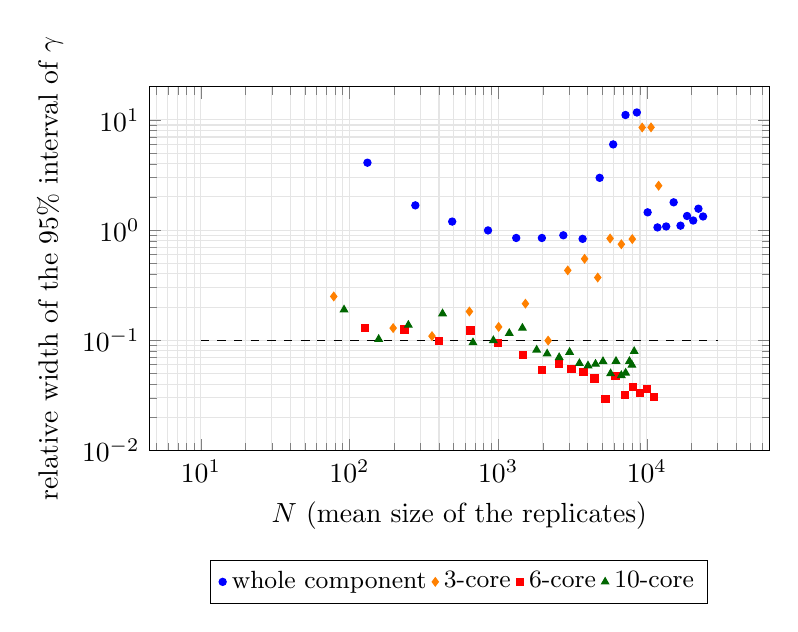
\begin{tikzpicture}
\begin{axis}[width=0.78\textwidth,height=6.2cm,xmode=log,ymode=log,xlabel={$N$ (mean size of the replicates)},
ylabel={relative width of the 95\% interval of $\gamma$},legend style={font=\small,at={(0.5,-0.3)},anchor=north,legend columns=4},
grid=both,grid style={gray!20},ymax=20,ymin=0.01]
\addplot[only marks,mark=*,mark size=1.3pt,blue] coordinates {(132,4.091) (277.2,1.678) (490.6,1.195) (854.5,0.9935) (1323,0.8484) (1969,0.8482) (2745,0.8972) (3700,0.8332) (4818,2.982) (5941,5.996) (7191,11.09) (8573,11.69) (1.013e+04,1.45) (1.18e+04,1.058) (1.35e+04,1.079) (1.516e+04,1.788) (1.686e+04,1.097) (1.866e+04,1.343) (2.052e+04,1.222) (2.225e+04,1.564) (2.391e+04,1.33)};
\addplot[only marks,mark=diamond*,mark size=1.5pt,orange] coordinates {(78.35,0.2498) (196.7,0.129) (358.8,0.1091) (640.5,0.1824) (1008,0.1322) (1526,0.2149) (2169,0.09927) (2940,0.4308) (3816,0.5485) (4677,0.3713) (5663,0.8392) (6740,0.7441) (7990,0.8288) (9308,8.542) (1.068e+04,8.566) (1.201e+04,2.528)};
\addplot[only marks,mark=square*,mark size=1.3pt,red] coordinates {(127.7,0.1288) (234.8,0.1252) (398.8,0.09853) (652.8,0.1225) (1002,0.09401) (1476,0.07338) (1980,0.05362) (2576,0.06104) (3122,0.05519) (3752,0.05176) (4438,0.04494) (5271,0.02909) (6168,0.04734) (7112,0.032) (8063,0.0377) (9021,0.03342) (1.007e+04,0.03616) (1.118e+04,0.03064)};
\addplot[only marks,mark=triangle*,mark size=1.5pt,black!60!green] coordinates {(91.85,0.1894) (157.1,0.1023) (248.8,0.1374) (422.5,0.1745) (676.9,0.09536) (928.2,0.09965) (1188,0.1157) (1456,0.1292) (1816,0.08173) (2136,0.07549) (2573,0.06989) (3025,0.07798) (3521,0.06171) (4022,0.05883) (4519,0.06086) (5073,0.06427) (5709,0.04986) (6206,0.06455) (6738,0.04801) (7206,0.05055) (7646,0.06448) (7943,0.05966) (8225,0.07937)};
\addplot[dashed,black,domain=10:30000] {0.1};
\legend{whole component,3-core,6-core,10-core}
\end{axis}
\end{tikzpicture}
\caption{Relative width of the 95\% interval of $\gamma$ under edge resampling, one point per cut. The
dashed line is 10\%. The whole component and the 3-core stay above it; the 6-core and 10-core fall below
it near $10^3$ and $2\times 10^3$ nodes.}\label{fig:width}
\end{figure}

\begin{table}[t]
\centering
\caption{Scale $N^{*}$ (mean replicate size) from which the width of $\gamma$ stays at or below 10\%
under edge resampling. The core order $k$ is the minimum degree.}\label{tab:crossings}
\begin{tabular}{lrrr}
\toprule
graph & min degree & $N^{*}$ & min degree $/\ln N^{*}$ \\
\midrule
whole component & 1 & never (to 25,000) & \\
3-core & 3 & never (to 15,000) & \\
6-core & 6 & 1,002 & 0.87 \\
10-core & 10 & 1,816 & 1.33 \\
15-core & 15 & 1,380 & 2.07 \\
\bottomrule
\end{tabular}
\end{table}

\subsection{Relaxation times and windows}
Units are as in \Cref{tab:cuts}: $1/\gamma$ and $T_c$ in continuous time, $T = 2T_c$ in lazy steps at
$\varepsilon = 1/2$, and $\delta = 10\%$. On the whole component, from 2009 on, $1/\gamma$ is 87 to 219
(174 to 438 lazy steps), $T_c$ is 17,000 to 44,000 and $T$ is 35,000 to 87,000 lazy steps
(\Cref{tab:cuts}). At the 2026 cut $1/\gamma = 112$, $T_c = 22{,}395$ and $T = 44{,}790$, against 33,342
nodes. The lazy-step window $T$ is 1.3 to 11 times $N$ (11 times at the 2009 cut, 6 at 2015, 1.3 at 2026):
the bound asks for a window longer than the graph has nodes before an average is good to 10\%. A 20\% target needs a
quarter of that. For the 6-core, above 1,000 nodes, $1/\gamma$ is 3.2 to 10, $T_c$ is 640 to 2,000 and $T$
is 1,300 to 4,000; for the 10-core $T_c$ is 650 to 1,540 and $T$ 1,300 to 3,100. The relaxation time of
the whole component grew by a factor of 20 at the 2009 cut, and that of the cores did not. Because the
window is proportional to $1/\gamma$, one weakly attached group raises it by the same factor.

\begin{figure}[t]
\centering
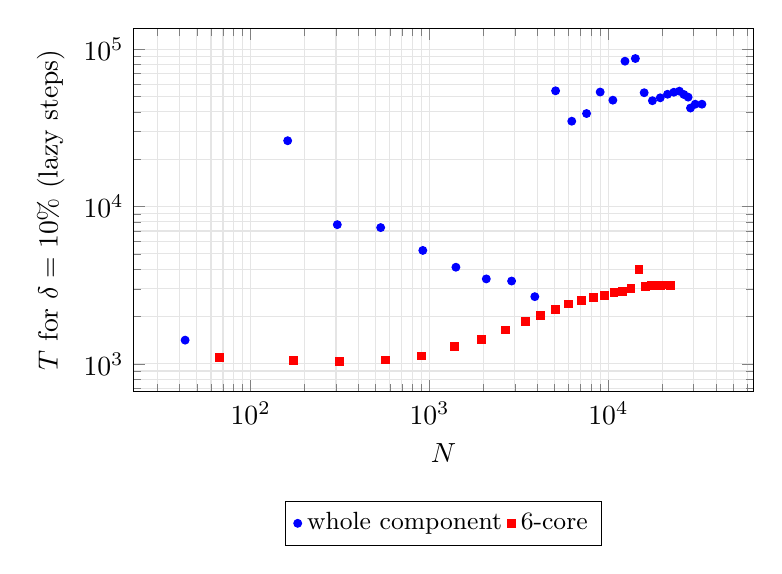
\begin{tikzpicture}
\begin{axis}[width=0.78\textwidth,height=6.2cm,xmode=log,ymode=log,xlabel={$N$},
ylabel={$T$ for $\delta=10\%$ (lazy steps)},legend style={font=\small,at={(0.5,-0.3)},anchor=north,legend columns=2},grid=both,grid style={gray!20}]
\addplot[only marks,mark=*,mark size=1.4pt,blue] coordinates {(43,1415) (161,2.624e+04) (305,7677) (533,7356) (917,5264) (1404,4116) (2076,3469) (2876,3363) (3878,2675) (5066,5.45e+04) (6239,3.492e+04) (7549,3.908e+04) (8995,5.353e+04) (1.059e+04,4.751e+04) (1.238e+04,8.407e+04) (1.415e+04,8.744e+04) (1.585e+04,5.298e+04) (1.762e+04,4.714e+04) (1.949e+04,4.919e+04) (2.141e+04,5.182e+04) (2.321e+04,5.335e+04) (2.493e+04,5.422e+04) (2.643e+04,5.162e+04) (2.791e+04,4.967e+04) (2.877e+04,4.235e+04) (3.058e+04,4.479e+04) (3.334e+04,4.479e+04)};
\addplot[only marks,mark=square*,mark size=1.4pt,red] coordinates {(67,1097) (173,1056) (313,1034) (569,1059) (906,1121) (1375,1282) (1945,1436) (2657,1641) (3424,1864) (4183,2038) (5048,2204) (6010,2403) (7083,2515) (8283,2628) (9528,2733) (1.074e+04,2828) (1.201e+04,2896) (1.337e+04,3024) (1.482e+04,3996) (1.613e+04,3096) (1.737e+04,3133) (1.845e+04,3162) (1.95e+04,3163) (2.012e+04,3173) (2.102e+04,3173) (2.223e+04,3169)};
\legend{whole component,6-core}
\end{axis}
\end{tikzpicture}
\caption{The window $T = 400/\gamma$ in lazy steps ($\varepsilon = 1/2$, $\delta = 10\%$) against $N$; the
continuous-time window $T_c$ is half of it. Above 5,000 nodes the whole component needs 1.3 to 11 times $N$;
the 6-core needs one to four thousand.}\label{fig:window}
\end{figure}

\subsection{The Hodge split of the citation flow}
\Cref{fig:hodge} shows the energy fractions of the flow against $N$. They settle early. From 2000
(43 nodes) the gradient fraction is 0.84 and then 0.80 to 0.83, the curl fraction 0.15 to 0.19 and
the harmonic fraction below 0.03; the harmonic fraction rises slowly from 0.002 to 0.027 as the graph grows.
The citation flow is mostly the gradient of a potential, which is close to a time order, with a stable
curl part from triangles whose three citations do not agree with any ranking.

\begin{figure}[t]
\centering
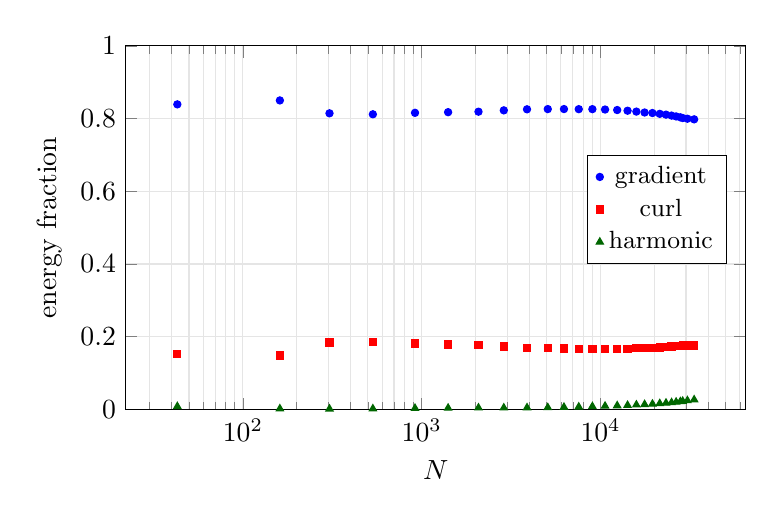
\begin{tikzpicture}
\begin{axis}[width=0.78\textwidth,height=6.2cm,xmode=log,xlabel={$N$},ylabel={energy fraction},
legend style={font=\small,at={(0.97,0.55)},anchor=east},grid=both,grid style={gray!20},ymin=0,ymax=1]
\addplot[only marks,mark=*,mark size=1.3pt,blue] coordinates {(43,0.839) (161,0.8498) (305,0.8144) (533,0.8117) (917,0.8157) (1404,0.8175) (2076,0.8188) (2876,0.8225) (3878,0.8254) (5066,0.826) (6239,0.8261) (7549,0.8258) (8995,0.8258) (1.059e+04,0.8248) (1.238e+04,0.8234) (1.415e+04,0.8215) (1.585e+04,0.8191) (1.762e+04,0.8166) (1.949e+04,0.8152) (2.141e+04,0.8129) (2.321e+04,0.8107) (2.493e+04,0.8081) (2.643e+04,0.8058) (2.791e+04,0.8034) (2.877e+04,0.8014) (3.058e+04,0.7995) (3.334e+04,0.7978)};
\addplot[only marks,mark=square*,mark size=1.3pt,red] coordinates {(43,0.1527) (161,0.1483) (305,0.184) (533,0.1863) (917,0.181) (1404,0.1786) (2076,0.1767) (2876,0.173) (3878,0.1698) (5066,0.1687) (6239,0.1676) (7549,0.1671) (8995,0.166) (1.059e+04,0.1659) (1.238e+04,0.1661) (1.415e+04,0.1671) (1.585e+04,0.1682) (1.762e+04,0.1696) (1.949e+04,0.1698) (2.141e+04,0.1707) (2.321e+04,0.1715) (2.493e+04,0.1731) (2.643e+04,0.1739) (2.791e+04,0.175) (2.877e+04,0.1758) (3.058e+04,0.1761) (3.334e+04,0.1755)};
\addplot[only marks,mark=triangle*,mark size=1.5pt,black!60!green] coordinates {(43,0.008324) (161,0.001984) (305,0.001598) (533,0.002026) (917,0.003292) (1404,0.003854) (2076,0.004472) (2876,0.004478) (3878,0.004776) (5066,0.005296) (6239,0.006269) (7549,0.007034) (8995,0.008199) (1.059e+04,0.009297) (1.238e+04,0.01048) (1.415e+04,0.01147) (1.585e+04,0.01266) (1.762e+04,0.01382) (1.949e+04,0.01494) (2.141e+04,0.01638) (2.321e+04,0.01773) (2.493e+04,0.01889) (2.643e+04,0.02034) (2.791e+04,0.02164) (2.877e+04,0.02276) (3.058e+04,0.02436) (3.334e+04,0.02675)};
\legend{gradient,curl,harmonic}
\end{axis}
\end{tikzpicture}
\caption{Gradient, curl and harmonic energy fractions of the citation flow at each cut.}\label{fig:hodge}
\end{figure}

\begin{table}[t]
\centering
\caption{Scale from which the width of each Hodge energy fraction stays at or below 10\%
(6 replicates per row; indicative to about a factor of two).}\label{tab:hodge}
\begin{tabular}{lrr}
\toprule
energy fraction & node sample (0.7) & edge resample \\
\midrule
gradient & 7 & 36 \\
curl & 1,402 & 856 \\
harmonic & never (to 25,000) & 2,744 \\
\bottomrule
\end{tabular}
\end{table}

The widths fall at much smaller scales than for $\gamma$ (\Cref{tab:hodge}). The gradient fraction is
within 10\% from the smallest sizes measured. The curl fraction is within 10\% from about 900 to
1,400 nodes, and the harmonic fraction from about 2,700 under edge resampling; under node
subsampling at 0.7 the harmonic width is 0.2 to 0.3 at 20,000 nodes. Energy fractions are averages
over all edges, so they are insensitive to a few weakly attached groups, while $\gamma$ is a
worst-case quantity.

\subsection{The contrast with a small personal corpus}
A graph of the size and shape of a small personal corpus was synthesized without reading any data:
38 nodes, 20 edges, one generation (18 parent nodes and 20 child nodes, each child holding one edge
to a uniformly drawn parent). Over 200 draws the graph has 8 to 16 components that contain an
edge (median 12), its largest component has 3 to 6 nodes (median 4) and minimum degree 1, and the whole
graph is a forest with $38 - 20 = 18$ components. Eigenvalue 0 therefore has multiplicity 18, the spectral
gap is 0, and the relaxation time and every window are infinite: a walk never leaves its component.
The largest component is a star with $\gamma = 1$, a property of the star that says nothing
about a corpus. Against the thresholds above, this graph is below $N^{*} \approx 10^3$ by a factor of
about 25 as a whole and 250 in its connected part, has minimum degree 1 where the
cores need about $\ln N$, and has no finite window.

For scale, two connected graphs on 38 nodes were measured the same way (200 edge resamples). A random
recursive tree (37 edges, mean degree over $\ln N$ of 0.54) has $\gamma = 0.026$, $T_c = 7{,}770$ and
$T = 15{,}540$ lazy steps and a width of 271\% (the resampled trees have 14 nodes on average). A tree plus random edges
to mean degree $2\ln N$ (138 edges, minimum degree 3) has $\gamma = 0.43$, $T_c = 465$ and $T = 930$ lazy steps and a
width of 47\%. Even connecting the corpus and giving it degree $2 \ln N$ leaves its macro quantities
far from the 10\% level that the real data reaches near $10^3$ nodes.

\section{Limitations}
\begin{itemize}
  \item One field and one source. A citation graph is strongly acyclic and time-oriented; a version
  chain, a hyperlink graph or a note corpus will differ. A Wikipedia sample was not collected.
  \item Reference lists in OpenAlex are incomplete for older works, and the in-field restriction
  deletes every reference to a work outside the field. This produces much of the degree-one structure
  that decides the whole-component result.
  \item The spectrum is of the symmetrized graph; the direction enters only the Hodge split. The
  walk whose relaxation time is reported is the undirected walk.
  \item Node subsampling and edge resampling measure sensitivity to deletion, not the sampling error
  of an unknown population. With 20 replicates (6 for the Hodge split) the extreme quantiles are
  coarse, and crossing scales are indicative to about a factor of two. Crossing scales are in the mean
  size of the replicates, which is smaller than the size of the graph resampled.
  \item The window assumes unit relative standard deviation of the observable and the sampled
  bound $2\sigma^2/(\varepsilon\gamma T)$ with $\varepsilon = 1/2$ (equivalently $2\sigma^2/(\gamma T_c)$); a particular observable may need less.
  \item The crossing is defined as staying under 10\% at every larger scale, which is stricter than
  the first dip.
  \item ARPACK can miss repeated eigenvalues; the smallest gap among $\lambda_3,\dots,\lambda_{20}$ was
  $1.5\times 10^{-6}$, so near repeats occur and only $\lambda_2$ and the first gaps are relied on.
  \item The last two years of OpenAlex are not comparable to the earlier ones.
\end{itemize}

\section{Future work}
Repeating the measurement on a graph with version chains (revisions of Wikipedia articles) would test
whether the minimum-degree reading carries over to a graph made of paths. A fresh draw
from a fitted growth model, in place of resampling the one observed graph, would separate sampling
error from sensitivity to deletion. A larger field and an API key would extend the scale axis by a
decade and allow cursor paging. The window bound could be checked directly by running the walk
and measuring the error of a time average of a degree-based observable against the window. The
$k$-cores are one remedy for the degree-one nodes; a weighting that downweights single citations
would keep all nodes.

\section{Conclusion}
On the citation graph of one field, the spectral gap of the whole largest component never has a 10\%
interval at any scale up to 25,000 nodes, because small groups on single citations set it and the
minimum degree is 1. On the 6-core and 10-core, with minimum degree about $\ln N$ at the crossing,
the interval under edge resampling is within 10\% from about 1,000 to 2,000 nodes, in line with the
degree condition of the concentration theorem. Windows for a 10\% average are 1.3 to 11 times $N$ lazy steps ($T$) on the
whole component and 1,300 to 4,000 on the cores. The Hodge energy fractions settle at much smaller
scales. A graph of 38 nodes and 20 edges in one generation lies below every threshold, and its
spectral gap is zero.

\bibliographystyle{plainnat}
\bibliography{refs}
\end{document}
